\documentclass[a4paper]{article}

%% Language and font encodings
\usepackage[english]{babel}
\usepackage[utf8]{inputenc}
\usepackage[T1]{fontenc}

%% Sets page size and margins
\usepackage[a4paper,top=3cm,bottom=2cm,left=3cm,right=3cm,marginparwidth=1.75cm]{geometry}

%% Useful packages
\usepackage{amsmath}
\usepackage{graphicx}
\usepackage[colorinlistoftodos]{todonotes}
\usepackage[colorlinks=true, allcolors=blue]{hyperref}

\newcommand{\github}{https://github.com/kauron/etsinf3/tree/master/CPA/lab2}
\newcommand{\gitname}[1]{\texttt{\href{\github /#1}{#1}}}
\newcommand{\gitline}[2]{\texttt{\href{\github /src/#1#2}{#1}}}

\newcommand{\m}[1]{\texttt{#1}}
\newcommand{\x}[1]{\m{#1}}
\renewcommand{\j}[1]{\m{#1}}

\title{Lab 2 Report}

\author{Carlos Santiago Galindo Jiménez\\Jesús Vélez Palacios}

\begin{document}
\maketitle
\section{Objectives}
To parallelize the execution of a program that reconstructs an image whose rows have been shuffled. To study different parallel and sequential improvements to the algorithm.

To examine the temporal cost of the different parallel and sequential versions. To determine the performance of the parallel versions with variable number of cores available to them and to detail the speedup and efficiency.

\section{Exercises\protect\footnotemark }
\footnotetext{All files are provided in the appropriate task in PoliformaT. However, the files are also on \href{\github}{GitHub} and they are linked through the report. These files will be exactly equal to those sent.}
\begin{enumerate}
    \item Time the method encaja. Completed with two calls to \m{omp\_get\_wtime()}. Source code: \gitline{encaja-e1.c}{\#L167}
    \item Parallelize each loop (if possible):
    \begin{enumerate}
        \item Loop \m{i} cannot be parallelized without altering greatly the code\footnotemark. Each iteration depends on the result of the previous one.
        \footnotetext{A possible parallel version could store all row in an array, each thread would pick a row as reference row to find its next row and then use the result as its new reference row, building shared linked lists (one per thread). When a thread has as result a row that is the head of another linked list, it would merge its linked list with the other, and would pick a new non-solved row as its new head. At the end, there would be a linked list containing the proper order of the rows, and a new loop would be needed to apply the result to the image matrix.}
        \item Loop \j can be parallelized, including the clause \m{private(x, distancia)}. The last \m{if} of the loop must be protected with a \m{critical} clause and the condition has to be rechecked after entering the critical section. Source code: \gitline{encaja-e2-pJ.c}{\#L118}
        \item Loop \x can also be parallelized, employing a \m{reduction(+:distancia)} clause to compute the distance correctly. Source code: \gitline{encaja-e2-pX.c}{\#L120}
    \end{enumerate}
    \item Improve the program by exiting loop \x if the partial sum surpasses the current minimum. Solved adding an \m{if} that stops the loop in that case. Source code: \gitline{src/encaja-e3.c}{\#L122}
    \item Parallelize each loop using the code from Exercise 3 (if possible):
    \begin{enumerate}
        \item Loop \j is parallelized in the same way as in Exercise 2. Source code: \gitline{encaja-e4-pJ.c}{\#L118}
        \item Loop \x cannot be parallelized using a \m{for} clause, as some iterations may be cut short by the modification in Exercise 3. It must be parallelized as a \m{parallel} block and each iteration assigned manually to the different threads. We have decided to assign the first iteration of each thread to \m{omp\_get\_thread\_num()} and to increment each thread's counter (\x) by \m{omp\_get\_num\_threads()}. It still needs a \m{reduction(+:distancia)} clause. Source code: \gitline{encaja-e4-pX.c}{\#L120}
    \end{enumerate}
\end{enumerate}

\section{Theoretical analysis}
\label{sec:theoretical}
To understand properly the values obtained by timing the different programs, a few concepts must be defined:
\begin{itemize}
	\item \textbf{Overhead}: time that the system spends creating, activating and deactivating threads when entering and exiting parallel regions. This time increases with the increase of number of threads, though the computing time might be reduced. This increase is more noticeable if the parallel regions are so short that the overhead could be greater than the parallel speedup.
	\item \textbf{Speed-up}: relation between the parallel and sequential timings. Values greater than 1 mean an improvement and lower than 1, a worsening.
	\item \textbf{Efficiency}: relation between the speedup and the number of threads available. This signifies the amount that each thread contributed to the speedup.
\end{itemize}

Knowing that loop \j contains loop {x}, in Exercise 2, loop \j is expected to have better results than loop \x, because of their respective size (\x has only one instruction) and number of times they are executed ($i$ vs $\frac{i^2}{2}$). Probably loop \x will have overhead problems.

Exercise 3 provides a great improvement, as it cuts, on average, loop \x's iterations in half, and this change is propagated to Exercise 4, that will combine the improvements from both 2 and 3. In Exercise 4 the comparison between \x and \j will still be the same described in Exercise 2.

\section{Experimental analysis}
\subsection{Experiment environment and execution}
All the programs have been compiled and executed in the cluster provided by the university\footnote{\url{kahan.dsic.upv.es}}.

The job file \gitname{encaja.sh} compiles\footnote{See the associated \gitname{Makefile}}, executes and checks the result of all the exercises, printing the results in \m{csv} format. On top of that, it executes the parallel programs with 2, 4, 8, 16 and 32 threads.

The following tables show the results of each experiment. Please note that the time values in the following tables refer to the time used by the method \m{encaja}, not the whole program, which also includes reading and writing the file.

\begin{figure}[h]
	\centering
	\begin{tabular}{l r}
		Program            & Execution time \\ \hline
		\m{encaja-e1} 	   & 15.257217      \\
		\m{encaja-e3}      &  2.725587      \\ \hline
	\end{tabular}
	\caption{Sequential execution times}
	\label{fig:table-time-seq}
\end{figure}
\begin{figure}[h]
	\centering
	\begin{tabular}{l r r r r r}
		Program               & 2t        & 4t        & 8t        & 16t        & 32t        \\ \hline
		\m{encaja-e2-pJ} 	  & 6.938746  & 3.548883  & 1.970450  & 1.183996   &  0.726187  \\
		\m{encaja-e4-pJ} 	  & 1.439842  & 0.795035  & 0.496000  & 0.330912   &  0.256960  \\
		\m{encaja-e2-pX} 	  & 8.337415  & 5.464151  & 5.557857  & 8.197272   & 12.789012  \\
		\m{encaja-e4-pX}	  & 4.065065  & 4.217589  & 5.164125  & 8.656438   & 13.590685  \\ \hline
	\end{tabular}
	\caption{Parallel execution times}
	\label{fig:table-time}
\end{figure}
\newpage
\todo{check better alternative than newpage}

\subsection{Time comparison}
In both \j loops, the time tends to asymptotically approach 0 as the threads increase, whereas in both \x loops, time tends to infinity.

As shown in Figure \ref{fig:graph-time} and predicted in section \ref{sec:theoretical}, loop \j performs much better than loop \x in both versions. The overhead problem in loop \x is so great that with number of threads greater than 8, its results begin to worsen dramatically (still, \x is an increase respect to the sequential version).

Exercise 3 greatly improves over Exercise 1, and its parallel versions (Exercise 4 -over Exercise 2) return the best results for loop \j. Loop \x performs better than the initial sequential version, but much worse than Exercise 3.

\begin{figure}[h]
	\centering
	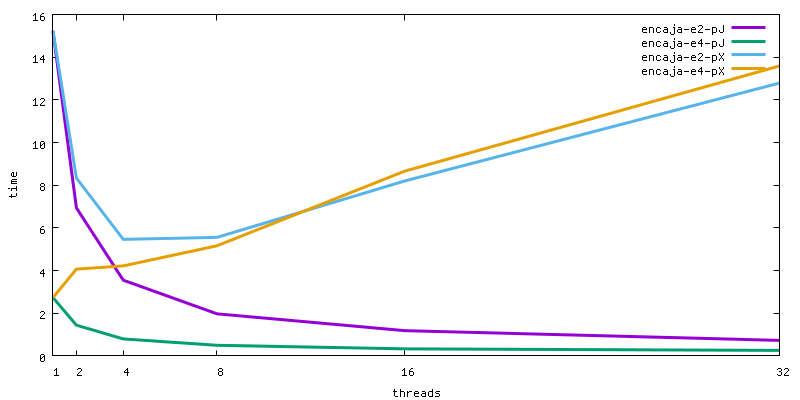
\includegraphics[width=\textwidth]{../img/time}
	\caption{Threads --- \unskip \, time graph \protect\footnotemark }
	\label{fig:graph-time}
\end{figure}
\footnotetext{The data in the graph for $threads=1$ represents the timing from the sequential versions of the program, and NOT the parallel versions with 1 thread.}


\subsection{Speed-up}
The speedup is computed as:
$$S(n,p)=\frac{t(n)}{t(n,p)}$$
Applying the previous formula with $t(n)=t_{encaja-e1}$ and $t(p,n)$ equal to each value in Figure \ref{fig:table-time} we obtain Figure \ref{fig:table-speedup}. In this case, all values are $>1$, therefore there is improvement in all cases respect with Exercise 1. The highest result is obtained by \m{encaja-e4-pJ} using 32 threads, being almost 60 times faster.
\begin{figure}[h]
    \centering
    \begin{tabular}{l r r r r r}
        Program               & 2t       & 4t       & 8t       & 16t      & 32t      \\ \hline
        \m{encaja-e2-pJ}	  &  2.19624 &  4.29407 &  7.73384 & 12.87090 & 20.98510 \\
        \m{encaja-e4-pJ} 	  & 10.58390 & 19.16790 & 30.72410 & 46.05190 & 59.30550 \\
        \m{encaja-e2-pX}	  &  1.82780 &  2.78893 &  2.74191 &  1.85905 &  1.19158 \\
        \m{encaja-e4-pX}	  &  3.74881 &  3.61323 &  2.95096 &  1.76044 &  1.12129 \\ \hline
    \end{tabular}
    \caption{Speedup}
    \label{fig:table-speedup}
\end{figure}

An interesting speedup to compute would be that of Exercise 4 respect to Exercise 3. This gives answers the question: How better can Exercise 3 be if parallelized? The answer lays on Figure \ref{fig:table-speedupR3}. The eye-catching situation is the loop \x's row, in which all values are $<0$, and therefore showing that parallelizing loop \x provides no improvement respect to the sequential version. The apparent betterment shown in Figure \ref{fig:table-speedup} is respect to the initial program. The threads --- \unskip \, time graph in Figure \ref{fig:graph-time} clearly shows that the performance of \m{encaja-e4-pX.c} (yellow) is below all other versions.

In the graph in Figure \ref{fig:graph-speedup} one can appreciate the scale of the improvements of the different versions, with the parallelization of loop \j in Exercise 4 greatly exceeding all others 2 or 3 times over. The almost flat lines at the bottom of the graph that show the speedup of loop \x demonstrate how insignificant the improvement is respect to loop \j.

\begin{figure}[h]
    \centering
    \begin{tabular}{l r r r r r}
        Program               & 2t       & 4t       & 8t       & 16t      & 32t       \\ \hline
        \m{encaja-e4-pJ}	  & 1.898620 & 3.438490 & 5.511530 & 8.261170 & 10.638700 \\
        \m{encaja-e4-pX}	  & 0.672491 & 0.648171 & 0.529368 & 0.315802 &  0.201147 \\ \hline
    \end{tabular}
    \caption{Speedup of \m{encaja-e4} respect to \m{encaja-e3}}
    \label{fig:table-speedupR3}
\end{figure}

\begin{figure}[h]
    \centering
    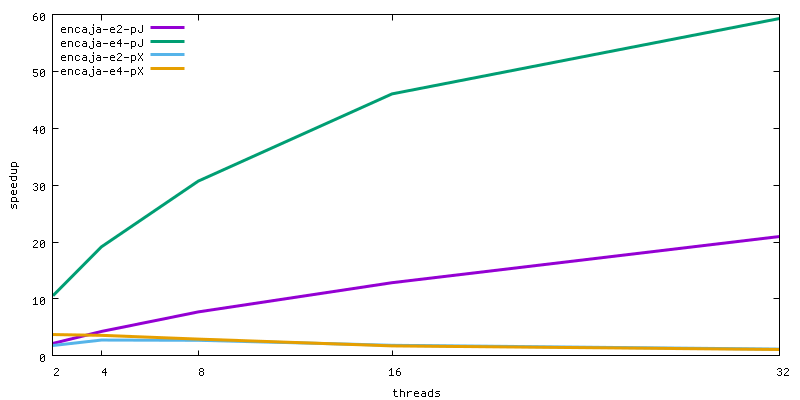
\includegraphics[width=\textwidth]{../img/speedup}
    \caption{Threads --- \unskip \, speedup graph}
    \label{fig:graph-speedup}
\end{figure}

\subsection{Efficiency}
The efficiency of a parallel program is computed as:
\begin{equation}
E(n,p)=\frac{S(n,p)}{p}
\end{equation}
where $p$ is the number of threads and $S(n,p)$ the speedup previously computed. Figure \ref{fig:table-efficiency} shows the efficiency values for exercises 2 and 4. As previously defined in section \ref{sec:theoretical}, higher values mean better results.

\begin{figure}[h]
	\centering
	\begin{tabular}{l r r r r r}
		Program 			  & 2t  	& 4t 	   & 8t 	  & 16t      & 32t 		\\ \hline
		\m{encaja-e2-pJ}	  & 1.09812 & 1.073520 & 0.966730 & 0.804431 & 0.655784	\\
		\m{encaja-e4-pJ}	  & 5.29195 & 4.791970 & 3.840510 & 2.878240 & 1.853300	\\
		\m{encaja-e2-pX}	  & 0.91390 & 0.697233 & 0.342739 & 0.116191 & 0.037237 \\
		\m{encaja-e4-pX}	  & 1.87441 & 0.903308 & 0.368870 & 0.110028 & 0.035040 \\ \hline
	\end{tabular}
	\caption{Efficiency}
	\label{fig:table-efficiency}
\end{figure}

As with previous measurements, loop \x approaches 0 with the increase of thread amount.

\begin{figure}[h]
    \centering
    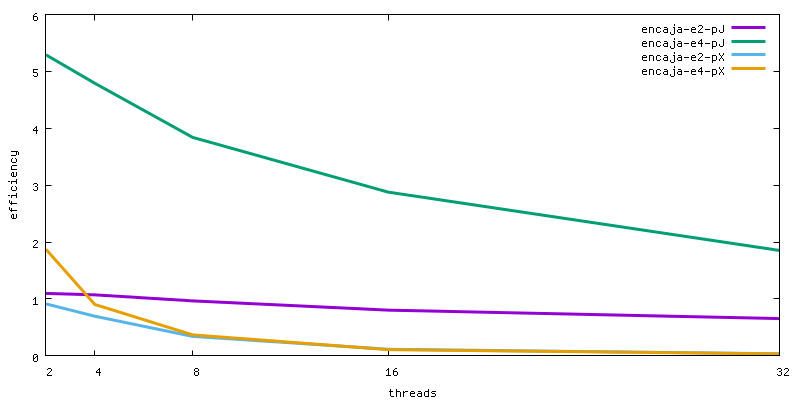
\includegraphics[width=\textwidth]{../img/efficiency}
    \caption{Threads --- \unskip \, efficiency graph}
    \label{fig:graph-efficiency}
\end{figure}

\section{Conclusions}\todo{txus' job}
This laboratory practice is an extensive walk-through of OpenMP and parallelization techniques and best practices. In these weeks we have learned that:\todo{maybe remove this}
\begin{itemize}
    \item Some loops can be parallelized, some cannot.
    \item Thread overhead may become a problem with inner loops.
    \item Clever changes to sequential algorithms can outperform simpler parallel ones.
    \item Appropriate control structures for critical sections and shared, private variables.
\end{itemize}


\end{document}

